\documentclass[tikz,border=10pt]{standalone}
\usepackage{tikz}
\tikzset{%
  big arrow/.style={
    decoration={markings,mark=at position 1 with {\arrow[scale=1.5,#1]{>}}},
    postaction={decorate},
    shorten >=0.4pt},
  big arrow/.default=black,
  point/.style={circle,inner sep=1.5pt,minimum size=1.5pt,draw,fill=#1},
  point/.default=red,
  edge/.style={line width=0.8pt,draw=#1},
  edge/.default=blue
}

\begin{document}
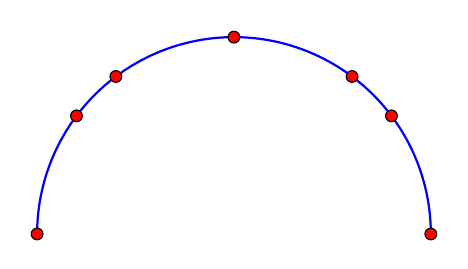
\begin{tikzpicture}[scale=0.5]

    % Draw grid and axes for context (optional, remove if not needed)
    %% \draw[thin, gray!30] (-6,0) grid (6,6);
    %% \draw[->, thick] (-6,0) -- (6,0) node[right] {$x$};
    %% \draw[->, thick] (0,0) -- (0,6) node[above] {$y$};

    % Draw the arcs and label them e_0 to e_5
    % Since it's a circle of radius 5, we use the exact angles for the paths.
    % v_0 (180°), v_1 (~143.13°), v_2 (~126.87°), v_3 (90°), v_4 (~53.13°), v_5 (~36.87°), v_6 (0°)

    \draw[edge] (-5,0) arc[start angle=180, end angle=143.13, radius=5]
        node[midway, above left, color=black] {};

    \draw[edge] (-4,3) arc[start angle=143.13, end angle=126.87, radius=5]
        node[midway, above left, color=black] {};

    \draw[edge] (-3,4) arc[start angle=126.87, end angle=90, radius=5]
        node[midway, above left, color=black] {};

    \draw[edge] (0,5) arc[start angle=90, end angle=53.13, radius=5]
        node[midway, above right, color=black] {};

    \draw[edge] (3,4) arc[start angle=53.13, end angle=36.87, radius=5]
        node[midway, above right, color=black] {};

    \draw[edge] (4,3) arc[start angle=36.87, end angle=0, radius=5]
        node[midway, above right, color=black] {};

    % Define the points with coordinates and labels
    % Coordinates:
    % v_0 = (-5,0), v_1 = (-4,3), v_2 = (-3,4), v_3 = (0,5), v_4 = (3,4), v_5 = (4,3), v_6 = (5,0)

    \node[point] (v0) at (-5,0) {};
    \node[point] (v1) at (-4,3) {};
    \node[point] (v2) at (-3,4) {};
    \node[point] (v3) at (0,5) {};
    \node[point] (v4) at (3,4) {};
    \node[point] (v5) at (4,3) {};
    \node[point] (v6) at (5,0) {};

\end{tikzpicture}
\end{document}
